\hypertarget{le-bonjour-du-village}{%
\section{Le bonjour du village !}\label{le-bonjour-du-village}}

\emph{Dimanche 06 mai 2018}

Les premières impressions du Liban (by Flo) :

\begin{itemize}
\tightlist
\item
  il fait chaud
\item
  il y a des voitures partout, notamment des SUV, et ça klaxonne pour
  tout et pour rien
\item
  ça sent la pollution dans la rue
\item
  on s'arrête régulièrement à des checkpoints militaires sur la route,
  plus généralement on note l'omniprésence de militaires
\item
  on se fait réveiller dès 5 heures du matin par des enfants qui jouent
  au foot dans la rue ou par la douce voix de l'épicier d'en face qui
  s'énerve sur tout le monde
\item
  c'est plein d'affiches politiques avec les têtes des candidats (le
  concours "ma binette partout"), ce qui s'explique par la tenue des
  élections législatives aujourd'hui
\end{itemize}

\begin{figure}
\centering
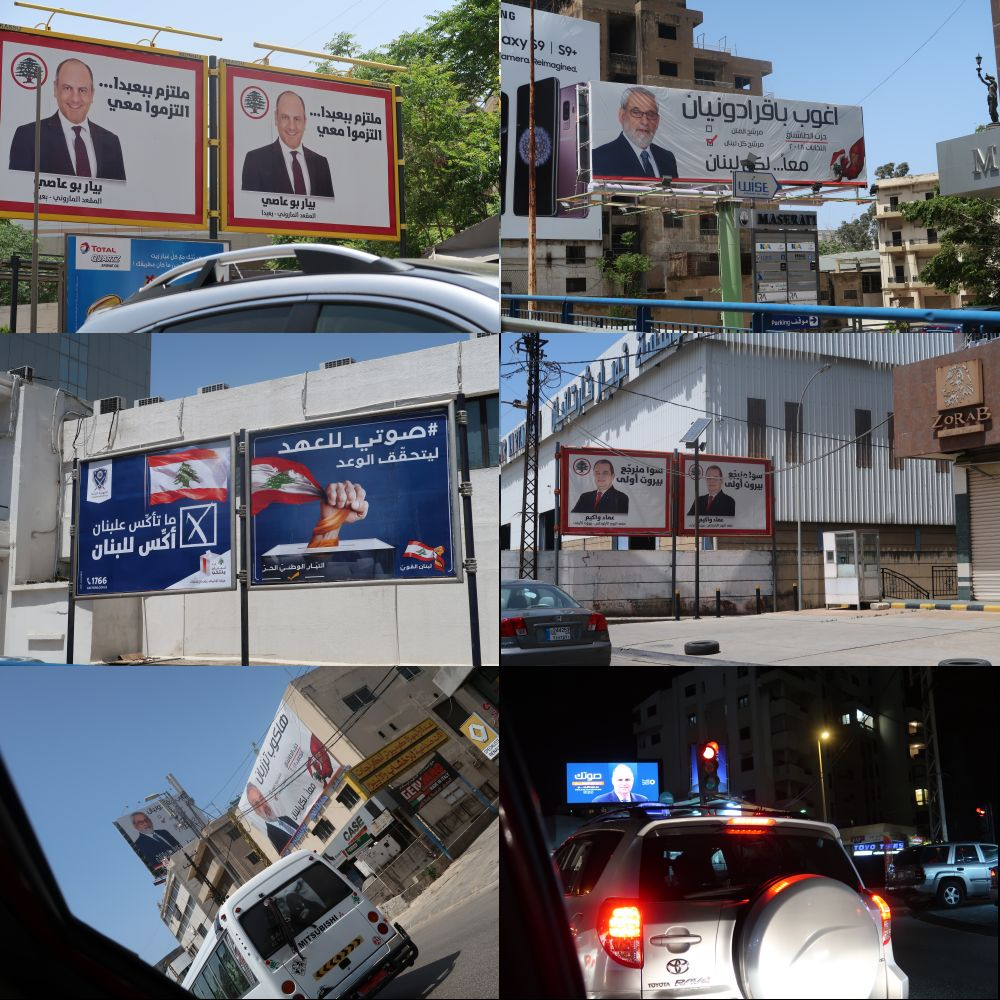
\includegraphics{images/20180506_politique.jpg}
\caption{Un échantillon d'affiches électorales libanaises.}
\end{figure}

Pour ne pas déséquilibrer le tableau, il faut rajouter deux choses : la
nourriture, qui est délicieuse (petit barbecue sur le toit pour nous
recevoir), et l'accueil adorable qui nous est reservé par la famille
d'Elida. De quoi envisager sereinement les prochains jours.

\begin{figure}
\centering
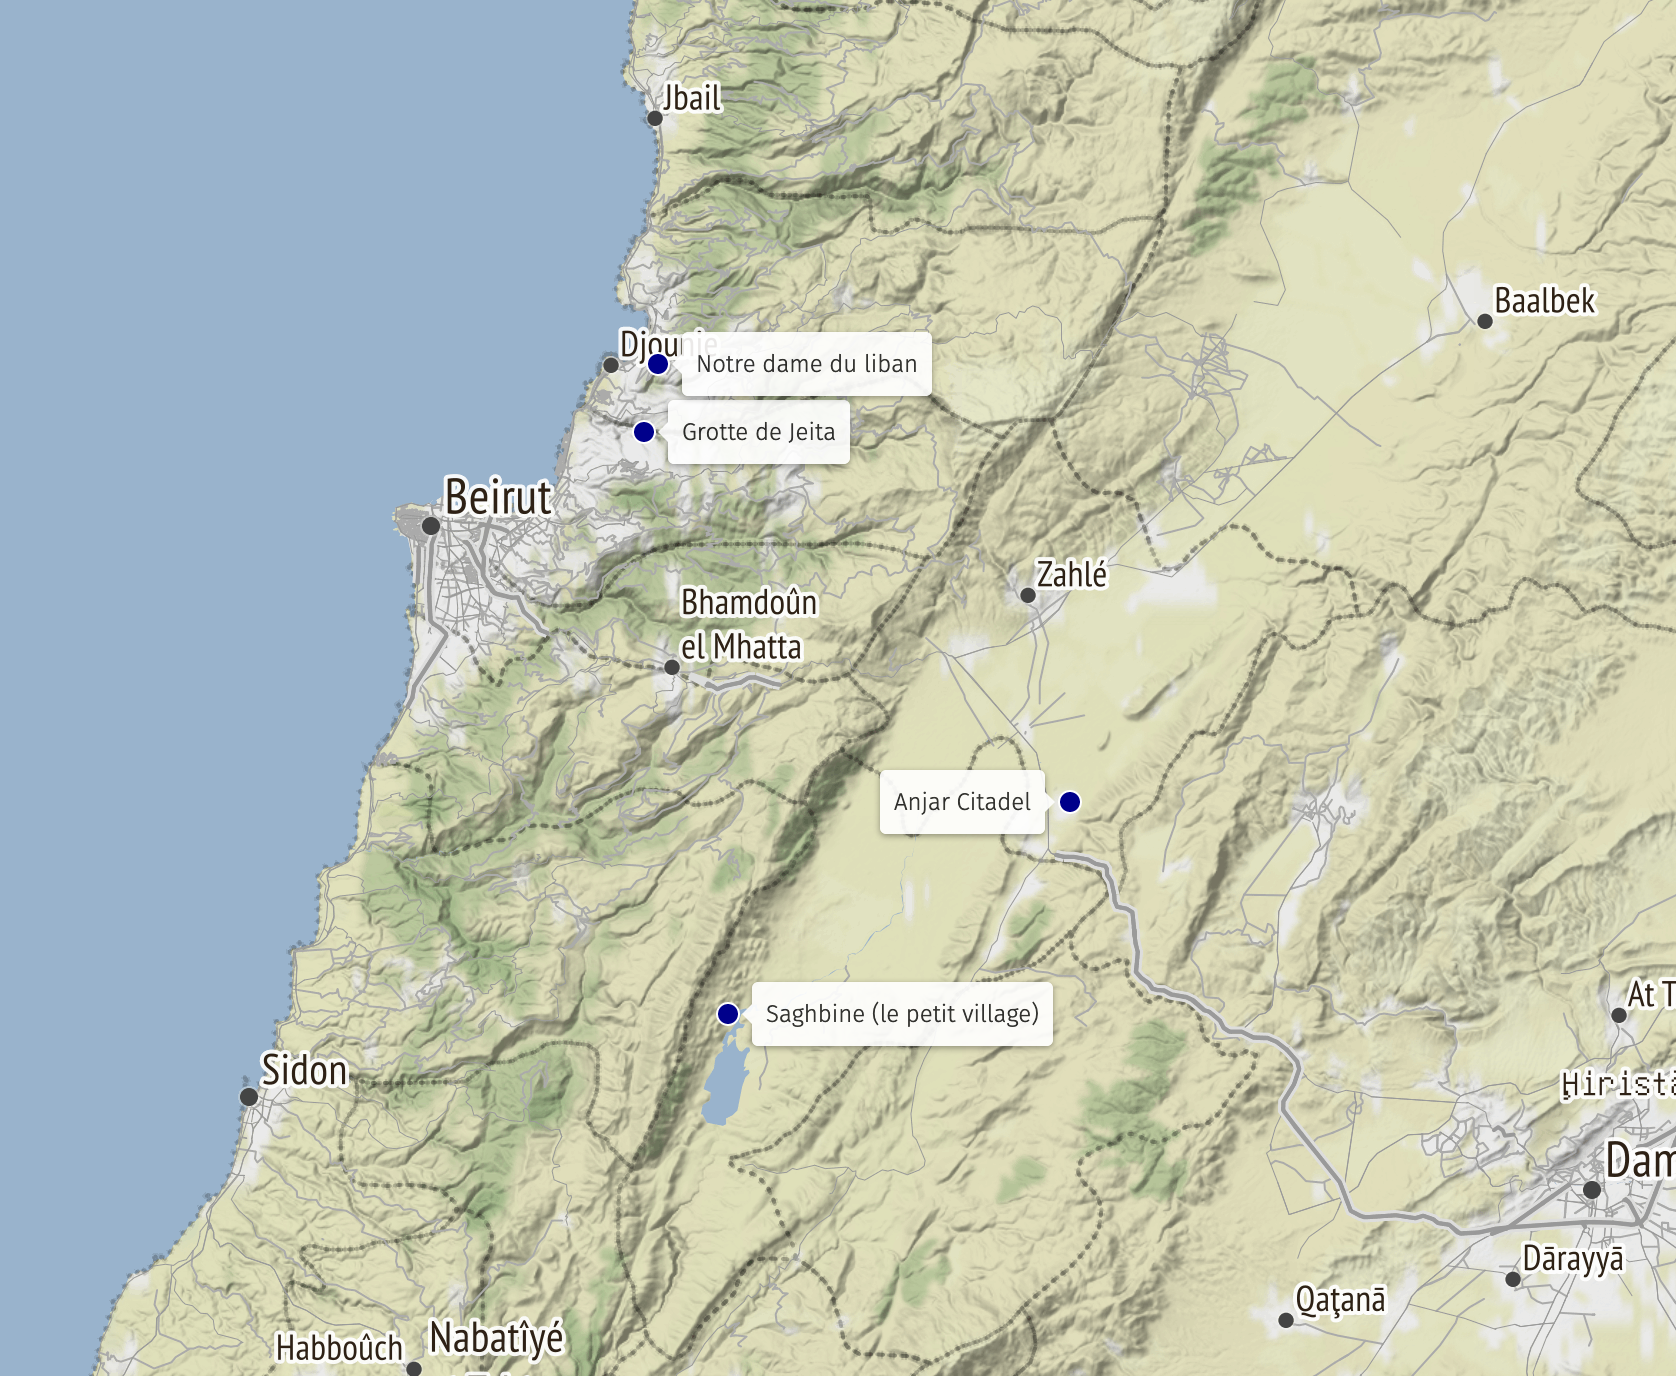
\includegraphics{maps/Liban1.png}
\end{figure}

Nous avons passé deux jours à Beyrouth, ce qui nous a donné
l'opportunité de commencer les visites au pas de course : les grottes de
Jeita, Notre Dame du Liban (NDDL pour ceux qui connaissent), le port de
Byblos.

\begin{figure}
\centering
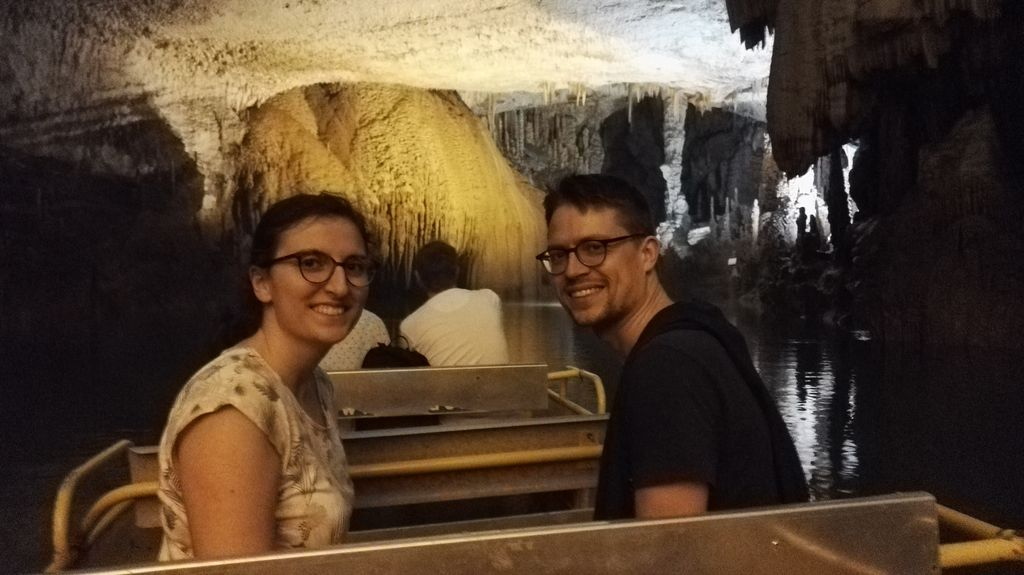
\includegraphics{images/20180506_Jeita.jpg}
\caption{Les grottes de Jeita, impressionnantes (photo volée exclusive,
bakchiche à la clé pour braver l'interdiction de photographier, on se
fait vite aux coutumes locales ;) )}
\end{figure}

Nous sommes maintenant à Saghbine, un petit village de la Bekaa de
l'ouest, une vallée coincée entre la chaîne montagneuse du mont Liban et
celle de l'anti-Liban (en face, quoi \^{}\^{}). Sur le chemin, nous
avons fait un détour par la ville d'Anjar (voir les photos de ruines
Omeyyades dans le style byzantin ci-dessous).

Ambiance politique aujourd'hui, on reste à l'écart et on vous tient au
courant !

\emph{Florian et Elida}

\hypertarget{commentaires}{%
\subsection{Commentaires}\label{commentaires}}

\begin{itemize}
\item
  François Baqué, \emph{2018-05-08 06h57}

  Bonjour depuis la Provence où la météo reste bien variable et
  fraiche... mois de mai hyper calme avec tous nos ponts et viaducs...\\
  Merci pour votre reportage libanais, au pays des cèdres majestueux et
  millénaires.\\
  Irez-vous à Byblos ? Ruines entremêlées sur 2000 ans d'histoire : des
  phéniciens aux croisés puis aux temps modernes !\\
  Vous êtes au cœur de l'origine de notre civilisation méditerranéenne :
  le barycentre (on reste dans les maths ?) de la culture mondiale
  actuelle (hors Chine : chaque chose en son temps).\\
  A très bientôt.\\
  François
\item
  Florian LB, \emph{2018-05-09 09h43}

  Bonjour François, merci pour ton message. Nous sommes passés en coup
  de vent à Byblos, mais nous y retournerons sans doute. Effectivement,
  les traces historiques sont très nombreuses au Liban et elles
  s'étalent sur des centaines et des centaines d'années, à ne plus
  savoir quelle époque on est en train de regarder. Concernant la météo,
  elle s'est nettement rafraîchie dans la vallée de la Bekaa depuis les
  lignes écrites ci-dessus...\\
  A bientôt,\\
  Florian
\end{itemize}
